\documentclass[tikz]{standalone}
\usepackage{tikz}
\usetikzlibrary{intersections,calc,quotes,angles}
\usepackage{tkz-euclide}
\begin{document}

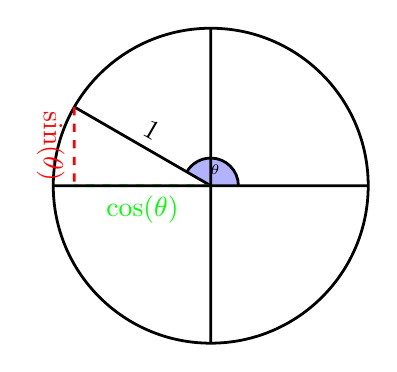
\begin{tikzpicture}[transparency group=knockout]

  \draw (2,0) arc[start angle=0, end angle=360, radius=2];
  \coordinate (A) at (0,0);
  \coordinate (B) at (2,0);
  \coordinate (C) at ({-sqrt(3)},{sqrt(1)});

  \draw pic[draw,fill=blue!30,angle radius=10,"$\theta$",font=\tiny] {angle=B--A--C};    
  
  \draw (0,0) --  ({-sqrt(3)},{sqrt(1)}) node[above,midway,sloped] {$1$};
  \draw[dashed, red] ({-sqrt(3)},{sqrt(1)}) -- ({-sqrt(3)},0) node[below,midway,sloped] {$\sin(\theta)$};
  \draw[dashed, green] (0,0) -- ({-sqrt(3)},0) node[below,midway,sloped] {$\cos(\theta)$};

  \draw (-2,0) -- (2,0);
  \draw (0,-2) -- (0,2);
\end{tikzpicture}
\end{document}